\chapter{Анализ существующих методов автоматизации наземных транспортно-технологических средств}\label{ch:ch1}

\section{Обзор современных подходов к автоматизации рабочих процессов наземных транспортно-технологических средств}\label{sec:ch1/sec1}

Процессы работы наземных транспортно-технологических средств (НТТС\nomenclature{НТТС}{наземные транспортно-технологические средства\nomrefpage}) и методы их автоматизации.

Наиболее ярким и востребованным примером автоматизации в сфере НТТС является беспилотное транспортное средство (БТС\nomenclature{БТС}{беспилотные транспортные средства\nomrefpage}).

В мире существует более 30 компаний, чья деятельность так или иначе связана с разработкой БТС: Apple; Audi (Volkswagen Group); Baidu; BMW, Intel и Mobileye; Bosch; DAF, Daimler, Iveco, MAN, Scania, Volvo; Delphi; Ford; General Motors, Lyft; Google, Fiat Chrysler Automobiles; Honda; Hyundai; Jaguar Land Rover; Mercedes-Benz (Daimler AG); Microsoft; Nissan, Renault; Nvidia; PSA Groupe; Tata Elixsi; Tesla; Toyota; Uber; Volkswagen; Volvo; Yutong и др.

Сегодня повышенное внимание к концепции создания БТС наблюдается и в российской автомобильной промышленности. Такие отечественные автопроизводители, как КамАЗ, Волгабас, Яндекс, ФГУП НАМИ и Кировский завод, ведут проекты по созданию БТС в партнерстве с разработчиками систем автоматического управления (Google, Uber, Baidu, Cognitive Technologies, КБ Аврора и другие).

Анализ показывает, что разработка БТС происходит по двум основным направлениям:

\begin{itemize}
    \item внедрение и расширение функциональности различных систем помощи водителю (которыми в настоящее время серийно комплектуются автомобили всех классов);
    \item создание способов и систем управления полностью БТС (которые в настоящее время находятся на стадии испытаний опытных образцов, в том числе эксплуатационных).
\end{itemize}

На рисунке~\cref{fig:patent} представлена динамика разработок наземных БТС, усовершенствованных систем помощи водителю (ADAS\nomenclature{ADAS}{Advanced Driver-Assistance Systems, усовершенствованная система помощи водителю\nomrefpage}) и их компонентов за рубежом.

\begin{figure}[ht]
    \centerfloat{
        \includegraphics[scale=0.5]{views/patent.png}
    }
    \caption{Динамика патентования за рубежом наземных БТС, систем ADAS и их компонентов в целом и раздельно за период с 2010 по 2016 годы}\label{fig:patent}
\end{figure}

Для реализации автономного управления движением БТС наиболее активно ведутся разработки и патентуются системы управления движением, которые включают: блоки управления интеллектуальным шасси, системы технического зрения, обработки и передачи информации, системы навигации и ориентации (рисунок~\cref{fig:system}). 

\begin{figure}[ht]
    \centerfloat{
        \includegraphics[scale=0.5]{drawio/system.drawio.png}
    }
    \caption{Подсистемы автоматизированной системы управления БТС}\label{fig:system}
\end{figure}

Конкретным примером в сфере НТТС можно рассмотреть разработку Научно-технического центра ПАО «КАМАЗ» совместно со специалистами МГТУ им. Н. Э. Баумана: самосвал КАМАЗ-6559 (рисунок~\cref{fig:ypiter30}), предназначенный для карьерных работ в автономном режиме.

\begin{figure}[ht]
    \centerfloat{
        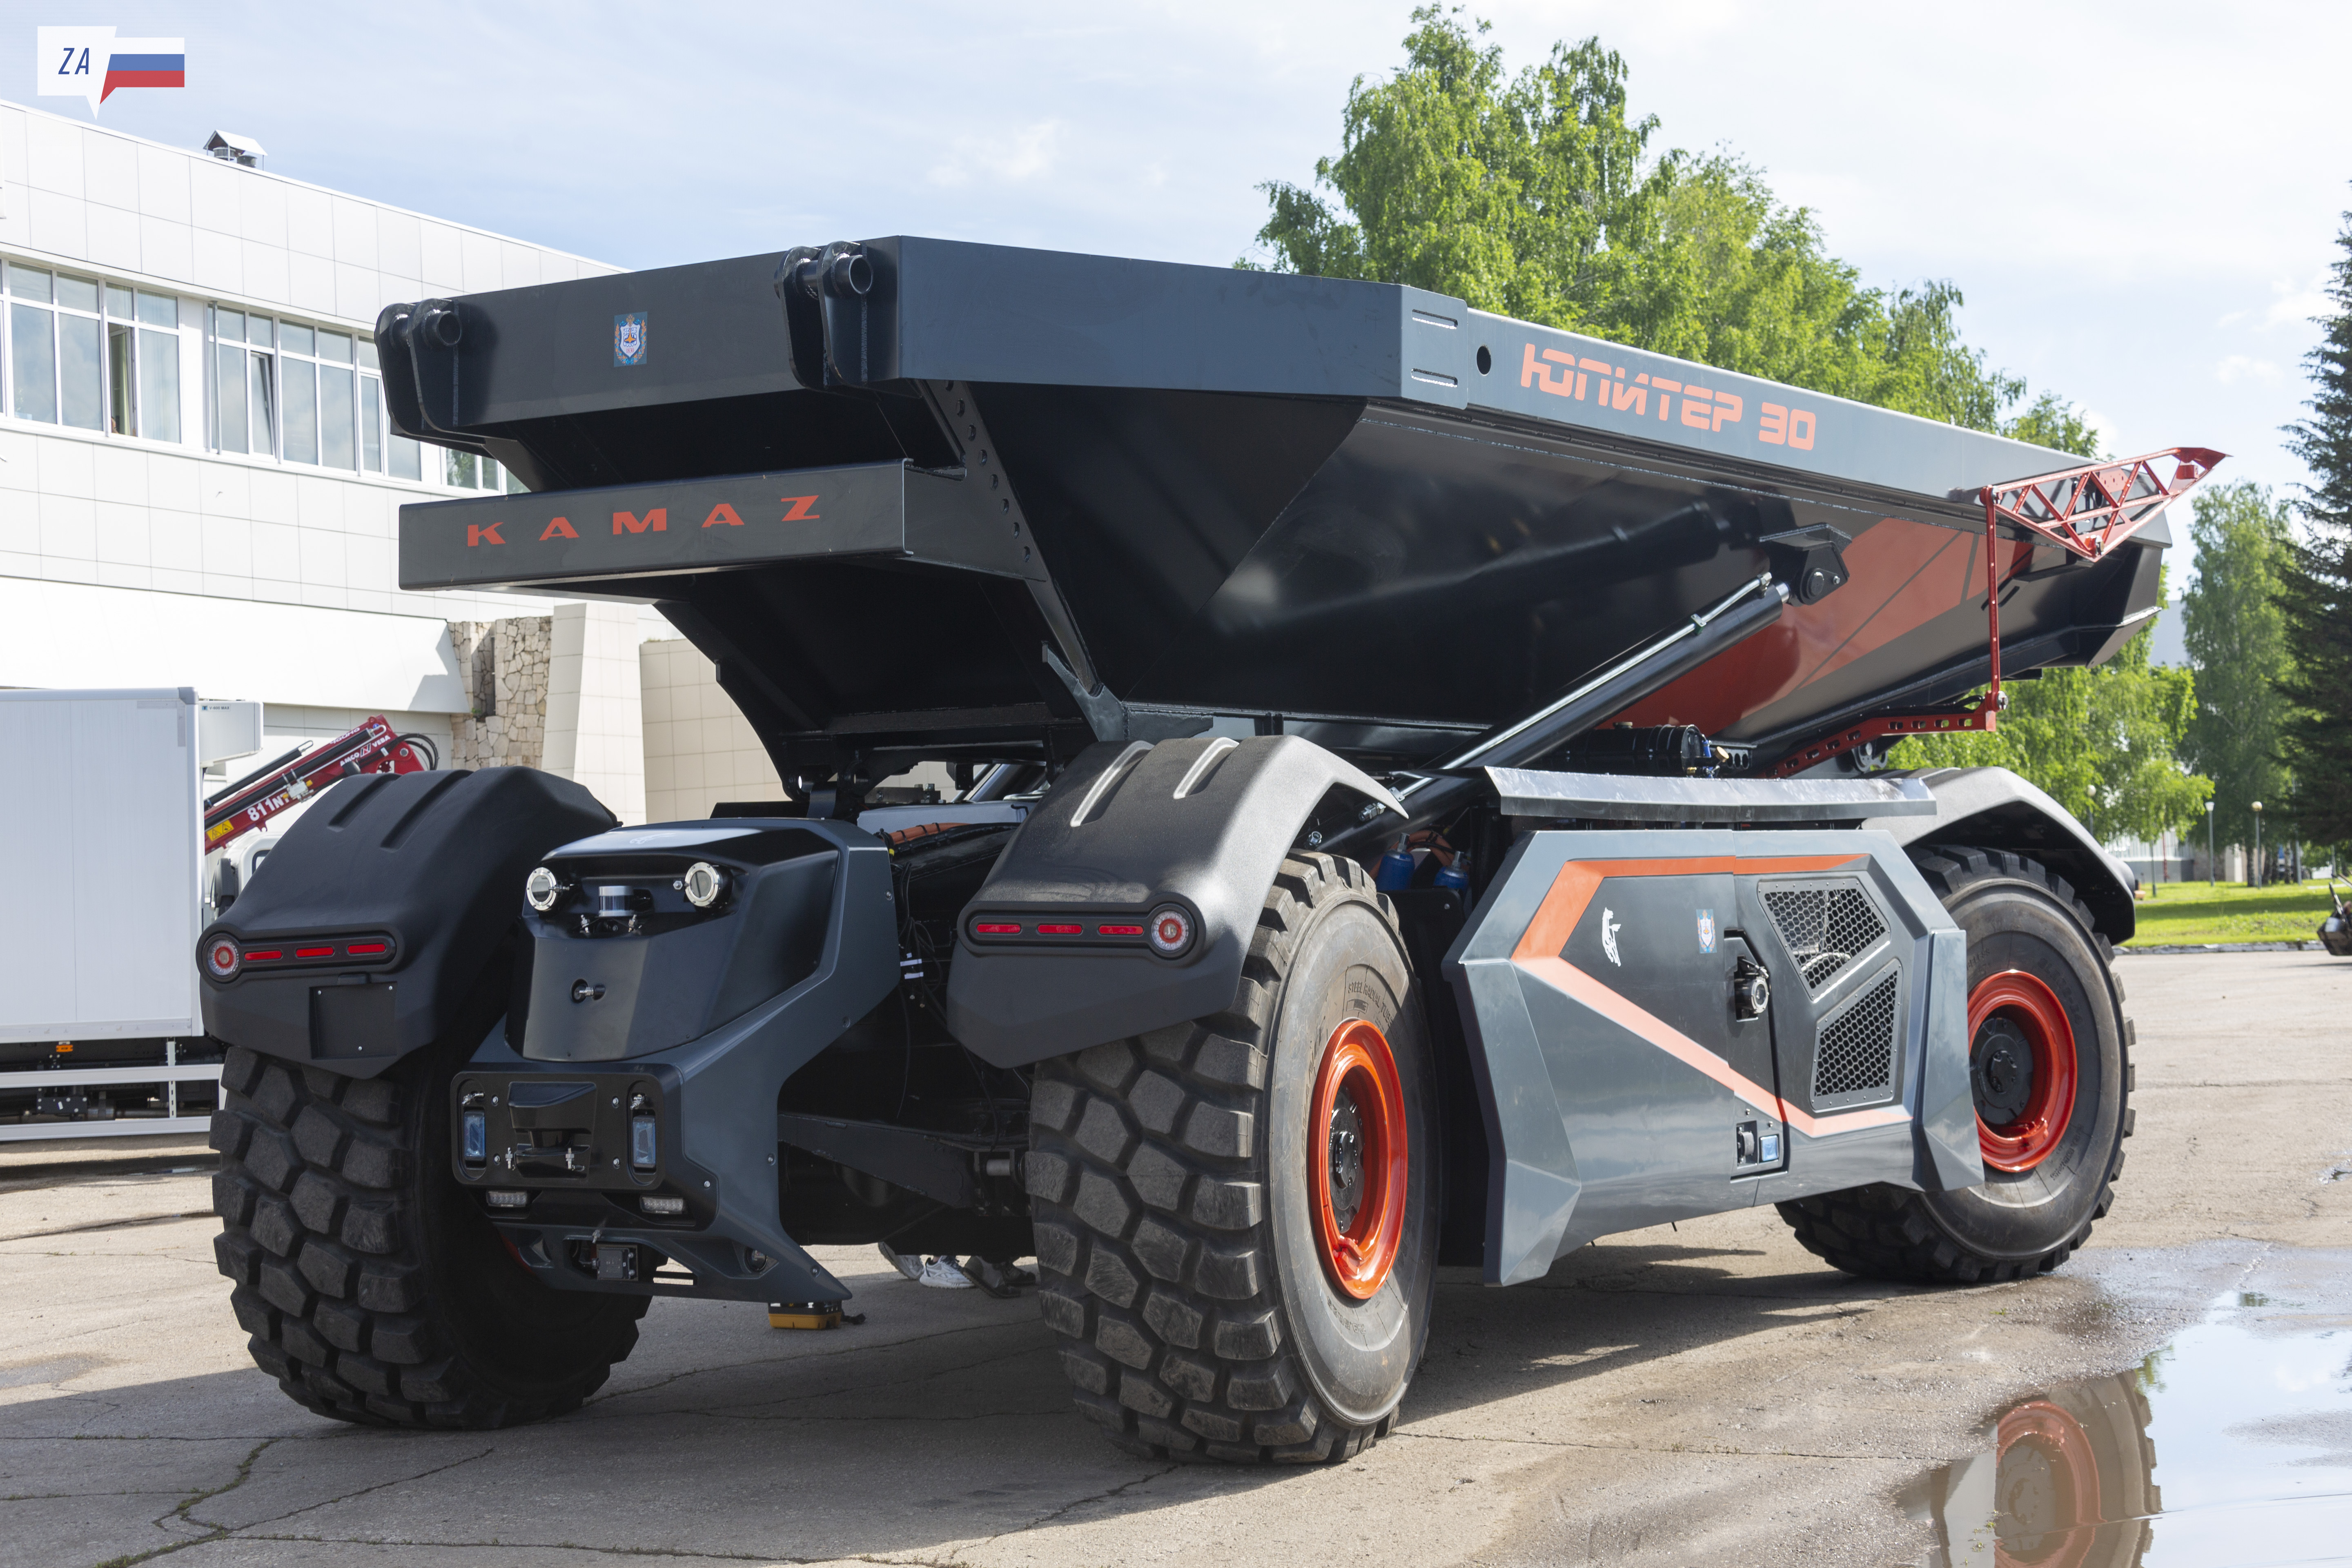
\includegraphics[scale=0.1]{views/kamaz.jpg}
    }
    \caption{Беспилотный КАМАЗ-6559 («Юпитер 30»)}\label{fig:ypiter30}
\end{figure}

БТС создан в рамках проекта «Создание семейства электромеханических беспилотных автомобилей-самосвалов большой грузоподъёмности в интересах добывающих отраслей промышленности РФ». Предназначен для перевозки разрыхлённой горной массы или руды по безлюдной технологии – без присутствия людей в опасной зоне работы большегрузных машин и экскаваторов. В связи с этой особенностью в конструкции автомобиля отсутствует кабина для водителя. НТТС изначально проектировался как автономное транспортное средство для работы в карьере. В нём установлены специальные, защищённые от пыли, грязи, влаги и вибраций видеокамеры, 2D- и 3D-лидары, ультразвуковые датчики, радары. Также имеются GSM-антенны и GPS/ГЛОНАСС навигация.

\section{Основные принципы автоматизации процесса работы наземных транспортно-технологических средств}\label{sec:ch1/sec2}

В общем виде системы управления движением БТС обеспечивают выполнение следующих операций:

\begin{itemize}
    \item получение и обработку данных с датчиков;
    \item объединение и согласование полученных данных;
    \item обработку изображений;
    \item определение препятствий, дорожных условий и автомобилей, расстояния до них;
    \item позиционирование БТС и определение текущего состояния системы;
    - реализацию автоматического управления скоростью БТС, траекторией (курсом) движения, автоматической реакцией на объекты, окружающие БТС;
    \item принятие решений на управляющие действия;
    \item управление исполнительными устройствами;
    \item формирование базы данных для последующего анализа.
\end{itemize}

\subsection{Системы управления и контроля}\label{subsec:ch1/sec2/sub1}

По степени автоматизации различают машины с механизированным управлением, с автоматизированным управлением и контролем на базе микропроцессорной техники, с автоматизированным управлением на расстоянии, с автоматическим управлением на базе микропроцессоров и мини-ЭВМ, строительные манипуляторы и роботы, а также роботизированные машины и комплексы \cite[с.~39]{Evtukov}.

\begin{figure}[ht]
	\centerfloat{
		\includegraphics[scale=0.5]{drawio/control.drawio.png}
	}
	\caption{Классификация систем управления и контроля машин}\label{fig:control_drawio}
\end{figure}

Системы управления предназначены для включения и выключения различных механизмов машин \cite[с.~109]{Evtukov}.
По назначению системы управления можно разделить на следующие: управлением двигателем; управление муфтами и тормозами; рулевое управление; управление рабочим органом (например, опускание и подъем отвала бульдозера или ковша скрепера, поворот отвала автогрейдера).

По конструкции системы управления строительных машин разделяют на механические, гидравлические, пневматические, электрические и смешанные (комбинированные), аналогично силовым приводам, но в отличие от которых в большинстве случаев в системах управления передаются значительно меньше силы.

Различают машины с механизированным и автоматизированным управлением. Автоматизированное управление и контроль рабочего процесса могут осуществляться на базе микропроцессоров и мини-ЭВМ, а также строительные манипуляторы и роботы, роботизированные машины и комплексы.

\subsection{Использование датчиков и сенсоров}\label{subsec:ch1/sec2/sub2}

С помощью различных датчиков обеспечивается сбор данных о состоянии окружающей среды. Датчики можно классифицировать на датчики внешней информации и внутренней \cite[с.~131]{Vlasov}. 

Датчики внутренней информации представляют собой в основном преобразователи механических параметров в электрические сигналы. Например датчики обратной связи по положению, скорости и ускорения.

\begin{figure}[ht]
    \centerfloat{
        \includegraphics[scale=0.5]{drawio/datchiki.drawio.png}
    }
    \caption{Классификация датчиков внешней информации}\label{fig:datchiki}
\end{figure}

Датчики внешней информации обеспечивают сбор информации об окружающем мире. Их можно разделить на две большие группы (рис.~\cref{fig:datchiki}): дистанционные и контактные. В свою очередь дистанционные датчики можно разделить на локационные и визуальные.

Локационные системы можно условно разделить на два класса: дальней и ближней локации. Первые могут быть построены с использованием ультразвуковых, лазерных и светолокационных датчиков.

Визуальные системы (технического, машинного зрения) относятся к числу наиболее сложных, но и наиболее универсальных средств очувствления НТТС (рис.~\cref{fig:kamaz},~\cref{fig:robot1},~\cref{fig:robot2},~\cref{fig:sensors}).

\begin{figure}[ht]
    \centerfloat{
        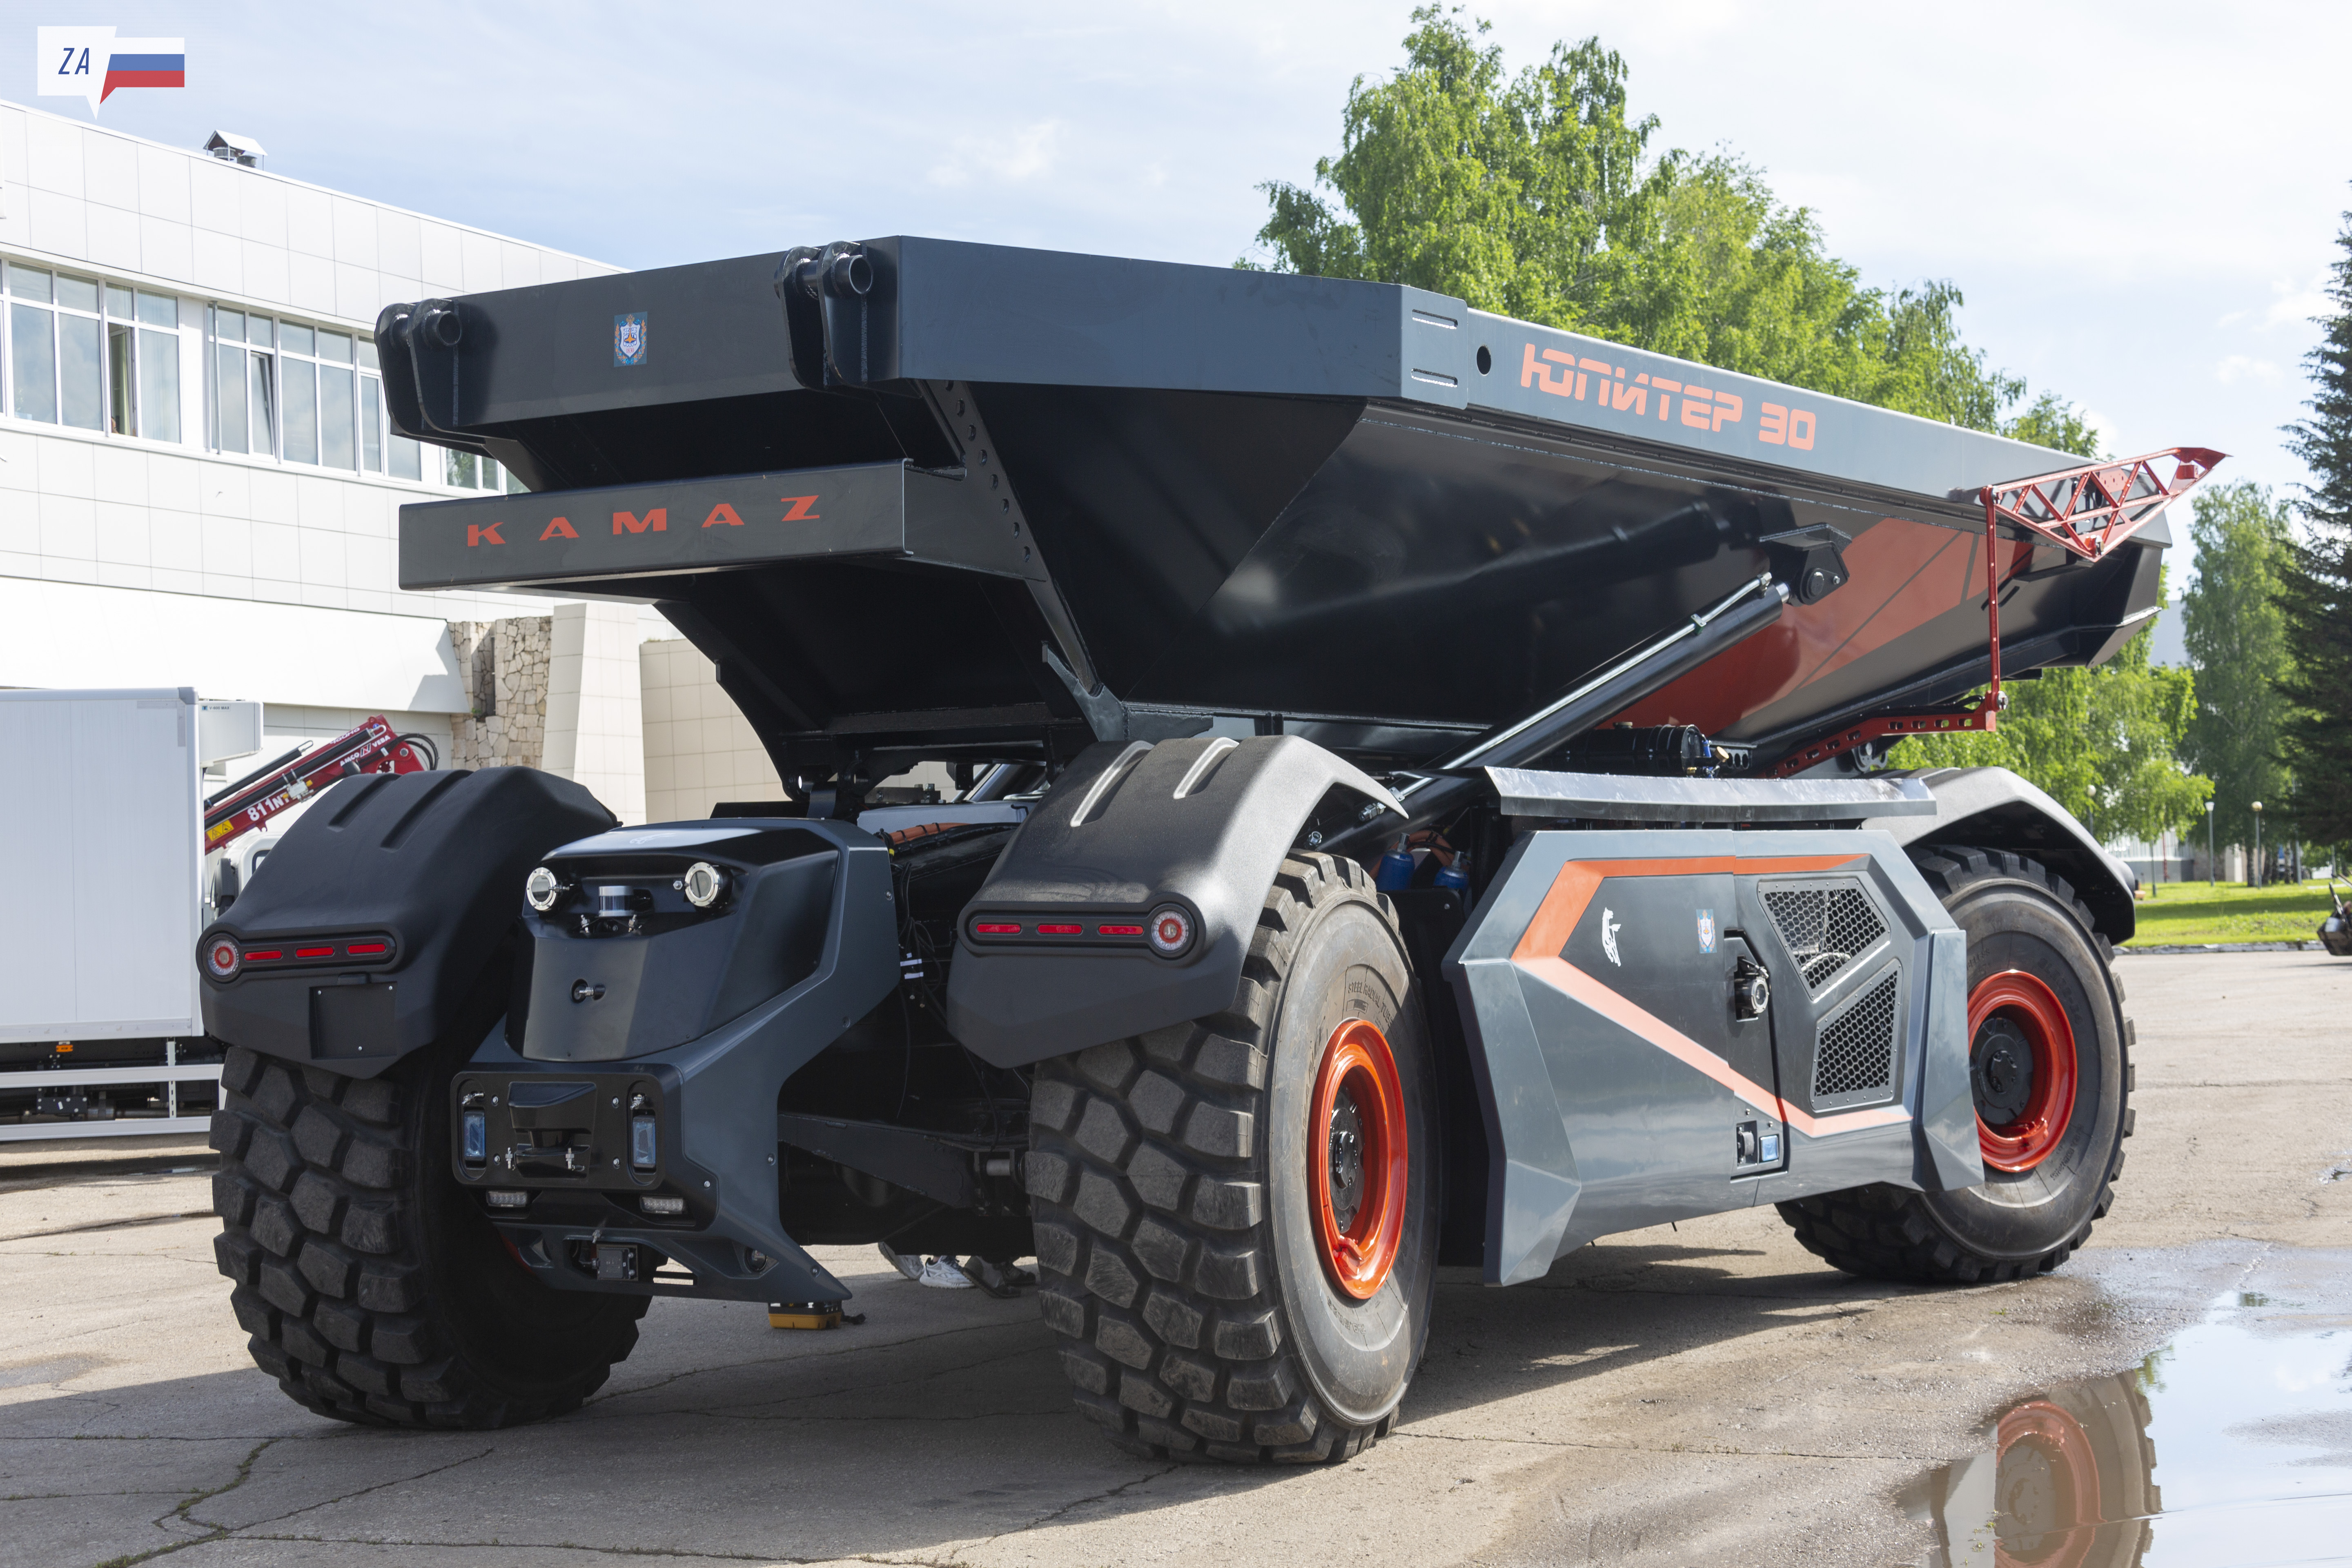
\includegraphics[scale=0.3]{views/kamaz.png}
    }
    \caption{Набор датчиков «Юпитер-30» ПАО «КАМАЗ»}\label{fig:kamaz}
\end{figure}

\begin{figure}[ht]
    \centerfloat{
        \includegraphics[scale=0.3]{views/robot1.png}
    }
    \caption{Набор датчиков автономного робота}\label{fig:robot1}
\end{figure}

\begin{figure}[ht]
    \centerfloat{
        \includegraphics[scale=0.4]{views/robot2.png}
    }
    \caption{Набор датчиков робота}\label{fig:robot2}
\end{figure}

\begin{figure}[ht]
    \centerfloat{
        \includegraphics[scale=0.6]{views/sensors.png}
    }
    \caption{Унифицированная схема взаимосвязи датчиков}\label{fig:sensors}
\end{figure}


Основными~\cite{confbib1} используемыми средствами машинного видения являются:

Лазерные дальномеры (лидары), которые измеряют расстояние до объектов. Результат работы лидара – объемная сцена из облака точек с геометрией объектов. Это средство выдает наибольшую точность, лучше всех работают на ровных поверхностях и почти не засвечиваются солнцем. При этом имеют высокое энергопотребление, относительно низкую частоту кадров, бегущий затвор и необходимость компенсировать его при обработке, а также работающие рядом лидары создают друг-другу помехи, которые не так просто компенсировать.

Радары для определения расстояния до объекта, его скорости и месторасположения. Радары меньше зависят от погоды и стоят намного дешевле лидаров. Главным отрицательным качеством является то, что плохо обнаруживаются неметаллические объекты, в том числе пешеходы.

Инфракрасные датчики для реагирования на фоновое инфракрасное излучение. Прибор регистрирует любое тепловое излучение.

Time-of-flight-камеры (ToF\nomenclature{ToF}{Time-of-flight-камеры\nomrefpage}) - видеокамеры, формирующие дальностное изображение. Используются для создания изображений, которые в качестве пикселей содержат оценки расстояний от экрана до конкретных точек наблюдения.

Стерео-камеры, построенные на имитации бинокулярного зрения человека с возможностью захватывать трехмерные изображения.

Пленоптические камеры, фиксирующие векторное поле световых лучей (световое поле). На основе картины светового поля может быть воссоздана наиболее полная информация об изображении, пригодная для решения различных задач компьютерной графики.

Обычные камеры с последующим анализом видео-потока с применением алгоритмов машинного обучения.

Так же можно приобщить разрабатываемый метод обмена данными о местоположении, скорости, направлении движения и другими данными между объектами.

Одновременно с этим, применение какого-либо одного средства недостаточно, так как получение комплексного видения окружающего мира роботами имеет сложности в виде:

\begin{itemize}
    \item темного времени суток;
    \item засветов от солнца и источников освещения;
    \item инфракрасного излучение солнечного света;
    \item осадков и грязи;
    \item множественности и вариативности подвижных окружающих объектов.
\end{itemize}

В связи с этим, средства машинного видения применяются комплексно, для компенсации недостатков друг-друга. Сравнительный анализ приведен в~таблице~\ref{tab:TableViews}.

\begin{table}[htbp]
    \centering
    \begin{threeparttable}
        \caption{Сравнительный анализ средств машинного видения}\label{tab:TableViews}%
            \begin{tabular}{{| p{3cm} || p{2cm} | p{2cm} | p{2cm} | p{2cm} | p{2cm} |}}
            \hline
            & ToF & Стерео & Пленопт. & Лидары & Радары \\ \hline
            Разрешение                 & \textit{Слабо}  & Средне & \textbf{\begin{tabular}[c]{@{}l@{}}Отлично\\ (сцена)\end{tabular}} & \begin{tabular}[c]{@{}l@{}}Средне\\ (сцена)\end{tabular} & \textit{Слабо}  \\ \hline
            Точность                    & Средне          & Средне          & \textit{Слабо}            & \textit{Слабо}  & \textbf{Высоко} \\ \hline
            Сложность ПО \nomenclature{ПО}{программное обеспечение\nomrefpage}                & \textbf{Слабо}  & Средне          & \textit{Высоко}           & \textit{Высоко} & \textbf{Слабо}  \\ \hline
            Работа в реальном времени   & \textbf{Высоко} & Средне          & Средне                    & Средне          & \textit{Слабо}  \\ \hline
            Стоимость                   & Средне          & Средне          & \textbf{Слабо}            & \textit{Высоко} & Средне          \\ \hline
            Производ-сть при слабом освещении & \textbf{Хорошо} & \textbf{Хорошо} & \textit{Плохо}            & \textit{Плохо}  & \textbf{Хорошо} \\ \hline
            Работа на открытом воздухе  & \textit{Плохо}  & \textit{Плохо}  & \textbf{Хорошо}           & \textbf{Хорошо} & \textbf{Хорошо} \\ \hline
            \end{tabular}
    \end{threeparttable}
\end{table}

Можно сделать вывод, что по разрешению лидируют пленоптические камеры, но все очень сильно зависит от сцены. По точности - лидары. По сложности обработки - «непосредственно» получают глубину только ToF и лидары. По частоте кадров конструктивно хороши ToF-камеры. При работе на открытом пространстве плохо работают ToF и камеры структурированного света.

Однозначно стоит в дальнейшем изучить и проанализировать использование совместно со средствами машинного видения такие методы, как:

\begin{itemize}
    \item определение местоположения в пространстве на основе глобальных систем позиционирования (GPS, ГЛОНАСС);
    \item получение данных от коллекторов навигационных данных (системы типа Яндекс-навигатор);
    \item заранее заложенные геопространственные данные;
    \item передачу управляющих сигналов внешними специализированными автоматизированными системами управления (по анализу данных с наружных камер наблюдения, управляющее воздействие регулятора и т.д.).
\end{itemize}


\subsection{Программное обеспечение для автоматизации}\label{subsec:ch1/sec2/sub3}

Программное обеспечение для автоматизации

\section{Координация автоматизированных НТТС}\label{sec:ch1/sec3}

Координация автоматизированных наземных транспортно-технологических средств

\section*{Выводы по главе}\label{sec:ch1/sec4}

Выводы

\FloatBarrier
